\documentclass[12px]{article}

\title{Lezione 20 Geometria I}
\date{2024-04-22}
\author{Federico De Sisti}

\usepackage{amsmath}
\usepackage{amsthm}
\usepackage{mdframed}
\usepackage{amssymb}
\usepackage{nicematrix}
\usepackage{amsfonts}
\usepackage{tcolorbox}
\tcbuselibrary{theorems}
\usepackage{xcolor}
\usepackage{cancel}

\newtheoremstyle{break}
  {1px}{1px}%
  {\itshape}{}%
  {\bfseries}{}%
  {\newline}{}%
\theoremstyle{break}
\newtheorem{theo}{Teorema}
\theoremstyle{break}
\newtheorem{lemma}{Lemma}
\theoremstyle{break}
\newtheorem{defin}{Definizione}
\theoremstyle{break}
\newtheorem{propo}{Proposizione}
\theoremstyle{break}
\newtheorem*{dimo}{Dimostrazione}
\theoremstyle{break}
\newtheorem*{es}{Esempio}

\newenvironment{dimo}
  {\begin{dimostrazione}}
  {\hfill\square\end{dimostrazione}}

\newenvironment{teo}
{\begin{mdframed}[linecolor=red, backgroundcolor=red!10]\begin{theo}}
  {\end{theo}\end{mdframed}}

\newenvironment{nome}
{\begin{mdframed}[linecolor=green, backgroundcolor=green!10]\begin{nomen}}
  {\end{nomen}\end{mdframed}}

\newenvironment{prop}
{\begin{mdframed}[linecolor=red, backgroundcolor=red!10]\begin{propo}}
  {\end{propo}\end{mdframed}}

\newenvironment{defi}
{\begin{mdframed}[linecolor=orange, backgroundcolor=orange!10]\begin{defin}}
  {\end{defin}\end{mdframed}}

\newenvironment{lemm}
{\begin{mdframed}[linecolor=red, backgroundcolor=red!10]\begin{lemma}}
  {\end{lemma}\end{mdframed}}

\newcommand{\icol}[1]{% inline column vector
  \left(\begin{smallmatrix}#1\end{smallmatrix}\right)%
}

\newcommand{\irow}[1]{% inline row vector
  \begin{smallmatrix}(#1)\end{smallmatrix}%
}

\newcommand{\matrice}[1]{% inline column vector
  \begin{pmatrix}#1\end{pmatrix}%
}

\newcommand{\C}{\mathbb{C}}
\newcommand{\K}{\mathbb{K}}
\newcommand{\R}{\mathbb{R}}


\begin{document}
	\maketitle
	\newpage
	\section{Teoremi vari su spazi Hermitiani e company}
	\begin{lemm}
		Sia $V$ uno spazio vettoriale su un campo $\R$\\
		Siano  $P,Q\in End(V)$ tali che $PQ=QP$. Allora, se  $V_\lambda$ è l'autospazio di autovalore $\lambda$ su $P$, risulta
		\[
		Q(V_\lambda)\subseteq V_\lambda
		.\] 
	\end{lemm}
	\begin{dimo}
		Sia $v\in V_ \lambda $ (cioè $P(v) = \lambda v)$. Dobbiamo vedere che $Qv\in V_ \lambda$.
		\[
		P(Q(v)) = (P\circ Q)(v) = (Q\circ P)(v) = Q( \lambda v) = \lambda Q(v)
		.\]
	\end{dimo}
	$(V,h)$ spazio Hermitiano (Spazio vettoriale complesso $h$ forma hermitiana definita positiva in $V$ )\\
	$\dim(V) < +\infty$
	 \begin{teo}
		Sia $(V,h)$ uno spazio hermitiano, $L\in End(V)$ operatore, sono equivalenti
		\begin{itemize}
			\item $L$ è normale (rispetto ad $h$)
			\item esiste una base ortonormale $B$ di  $V$ composta da autovettori per $L$
		\end{itemize}
	\end{teo}
	\begin{lemm}
		$(V,h)$ spazio hermitiano, $L\in End(V)$ normale\\
		sono equivalenti
		\begin{itemize}
			\item $Lv = \lambda v$
			\item  $L^\star v = \overline{ \lambda} v$
		\end{itemize}
		In particolare $ \lambda$ è l'autovalore per $L$ se e solo se $\overline{ \lambda}$ è autovalore per $ L^\star$ 
		\[
			V_ \lambda (L) = V_{\overline{ \lambda}}(L^\star)
		.\] 
	\end{lemm}
	\begin{dimo}
		Se $v = 0$ non c'è niente da dimostrare.\\
		Se $v \neq 0$ basta far vedere che se $v\in V_ \lambda (L)$ allora $v\in V_{\overline{ \lambda}}(L^\star)$. L'inclusione contraria segue da $L^{\star t} = L$
		 \[
		w\in V_ \lambda (L), \ \ v\in V_ \lambda (L)
		.\] 
		\begin{aligned}
			\hspace{80px}h(L^\star(v),w) &= h(v,L(w)) = h(v, \lambda w)\\
					&=\overline{ \lambda}h(v,w) = h(\overline{ \lambda}v,w)
		\end{aligned}\\
		\[
			h(L^\star(v) - \overline{ \lambda}v,w) = 0 \ \ \circledast
		\] 
		Per il lemma, siccome per ipotesi $L$ è normale, 
		 \[
		L^\star (v)\in V_\lambda (L), \ \ \overline{
		\lambda}v\in V_ \lambda (L)
		\] 
		\[
			\Rightarrow \ \ \ L^\star (v) - \overline{ \lambda} v\in V_ \lambda (L)
		\] 
		Quindi nella $\circledast$ posso prendere $w = L^\star (v) - \overline{ \lambda} v$, ottenendo 
		\[
			h(L^\star (v) - \overline{ \lambda} v, L^\star (v) - \overline{\lambda} v) = 0
		.\] 
		Poiché $h$ è definito positivo, segue\\
		\begin{aligned}
			&L^\star(v) - \overline{ \lambda}v = 0\\
			\text{cioè} \hspace{50px}  & L^\star (v) = \overline{ \lambda} v
		\end{aligned}\\
	\end{dimo}
	\textbf{Osservazione}\\
	Dal lemma segue $V_ \lambda(L) \perp V_\mu (L)$ se $ \lambda \neq \mu$
	\[
	v\in V_ \lambda, \ \ \ w\in V_\mu
	\] 
	\[
		\lambda h(v,w) = h( \lambda v,w) = h(Lv,w) = h(v,L^\star w) = h(v, \overline{\mu}w) = \mu h(v,w) \Rightarrow  h(v,w) = 0
	\]
	Dato che $ \lambda \neq \mu$
	\begin{dimo}[Teorema Spettrale]
		$1) \Rightarrow  2)$ Procediamo per induzione su $\dim V$,con base ovvia $\dim V = 1$ \\
		Supponiamo il teorema vero per gli spazi hermitiani di dimensione $\leq n-1$ e sia  $\dim_\C V = n$\\
		Sia  $v_1\in V$ un autovettore per $L$, che possiamo assumere di norma  $1$. Sia $V_1 = \C v_1, W = v_1^perp$.\\
		Allora $V = V_1 \oplus W$.\\
		Poiché $V_1$ è $L$-invariante (per costruzione) e $L^\star$-invariante per il lemma precedente, lo stesso accade per  $W$.\\
		Inoltre $L|_W\in End(V)$ è normale.\\
		Per induzione, esiste una base $h|_W$-ortonormale formata da autovettori per $L|_W$, sia $\{v_2,\ldots,v_n\}.$ Allora $\{v_1,\ldots,v_n\}$ è una base $h$-ortonormale di $V$ formata da autovettori per $L$.\\
		$2) \Rightarrow 1)$. Sia $B = \{v_1,\ldots,v_n\}$ una base $h$-ortonormale di autovettori per $L$. Allora\\
		\begin{aligned}
			\hspace{80px}&[L]^B_B = \bigwedge = \matrice{ \lambda_1  &\ldots& 0\\
				 0  & \ddots & 0\\
			 0  &\ldots & \lambda_n}\\
			    &[L^\star]^B_B = \overline{[L]_B^B}^t = \overline{\bigwedge}\\
			    &[L\circ L^\star]^B_B = [L]^B_B[L^\star]^B_B = \bigwedge\overline{\bigwedge}=\overline{\bigwedge}\bigwedge = [L^\star]_B^B[L]^B_B = [L^\star \circ L]_B^B
		 \end{aligned} \\
		 Poiché la mappa $A \rightarrow [A]^B_B$ è un isomorfismo tra
		 $End(V)$ e $M_{nn}(\C)$, segue 
		 \[
		 L\circ L^\star = L^\star \circ L
		 .\] 
		 cioè $L$ è normale
	\end{dimo}
	\textbf{Osservazioni}\\
	1. È essenziale che $h$ sia definita positiva.\\
	\[
	 h(x,y) = x^tH\overline{y} \ \ \ M = \matrice{1&0\\0&-1}
	.\] 
	non è definita positiva $h(\icol{0\\1},\icol{0\\1}) = -1$
	\[
		L_A:\C^2 \rightarrow\C^2 \ \ A = \matrice{0&i\\i & -2}
	.\] 
	Dico che $L_A$ è autoaggiunto, quindi normale\\
	\begin{aligned}
		\hspace{80px}&h(L_AX,Y) = h(X,L_AY)\\
		&(L_AX)^tH\overline{Y} = X^tH\overline{L_AY}\\
		&X^tA^tH\overline{Y} = X^tH\overline{A}\overline{Y} \ \ \forall X,Y\\
		&A^tH = H\overline{A}\\
		&\matrice{0&u\\i&-2}\matrice{1&0\\0&-1} = \matrice{1&0\\0&-1}\matrice{0&-i\\-i&-2}\\
		&\hspace{47px}\matrice{0&-i\\i&2} = \matrice{0&-i\\i&2}
	\end{aligned}
	Calcolo il polinomio caratteristico di $A$ 
	\[
		\det\matrice{t& -i\\-i & t + 2} = t(t+2) + 1 = (t+1)^2
	.\] 
		Ma $A\neq \matrice{-1&0\\0&-1}$, in particolare non è diagonalizzabile\\
		2. Vediamo in dettaglio il fatto che $L|_W$ è normale\\
		Ritornando alla dimostrazione del teorema spettrlae, osserviamo che se $W$ è $L$-invariante è anche $L^\star$-invariante.\\
		Infatti, se $V = \bigoplus_\lambda V_ \lambda(L)$ (per esercizio da dimostrare)\\
		\begin{aligend}
			$W &= \bigoplus_ \lambda (V_ \lambda(L)\cap W)$\\
			   &=\bigoplus_ \lambda (V_{\overline{ \lambda}}(L^\star)\cap W)
			
		\end{aligend}\\
		$=> W$ è $L^\star$-invariante\\
		Adesso osservo che $(L|_W)^\star = (L^\star)|_W$\\
		\begin{aligend}
			&(L\left|_{W)}\circ(L\right|_W)^\star = (L|_W)\circ(L^star|_W) = \\
			&(L\circ L^\star)|_W = (L^\star\circ L)|_W = (L^\star|_W) \circ L|_W = (L|_W)^\star\circ L|_W
		\end{aligend}\\
		\section{Richiami su spazi vettoriali duali}
		$V$ spazio vettoriale su $\K$ di dimensione finita
		 \[
		V^V = V^śtar = Hom(V,\K)
		.\] 
		sia $A\leq V$
		 \[
			 Ann(A) = A^\# = \{f\in V^\star | f(a) = 0 \ \ \forall a \in A\}
		.\] 
		\textbf{Osservazioni}\\
		1) $A^\# $ è un sottospazio\\
		2) $A^{\#\#} = <A>$ \\
		\begin{aligned}
			\hspace{100px}&i:V \rightarrow V^{\star\star}\\
			&v\in V, \ \ f\in V^\star\\
			& i(v)(f) = f(v)
		\end{aligned}\\
	$V,W$ spazi vettoriali di dimensione finita $f\in Hom_\K(V,W)$, $f^\star\in Hom_\K(W^\star,V^\star)$, la trasposta di f è definita con $\phi\in W^\star$\\
	\hspace{40px}$f^\star(\phi) = \phi\circ f \\
	$\text{ }\hspace{100px}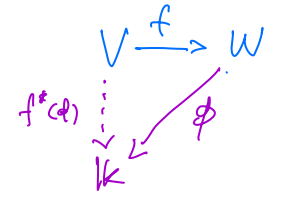
\includegraphics[scale=0.4]{funzione}\\
	\begin{defi}
	Definisco la  dualità standard su $V$ come 
	\[
	\langle \ , \  \rangle : V^\star\times V \rightarrow \K
	.\] 
	$\langle v, f \rangle = \langle f, v \rangle = f(v)$\\
	con questa proprietà
	\[
	\langle f(v), w^\star \rangle  = \langle v, f^\star(w^\star) \rangle 
	.\] 
\end{defi}
\hline \ \\
Ricordo che se $B = \{v_1,\ldots,v_n\}$ è una base di $V$ allora i funzionali $v_i^\star$ definiti da
 \[
	 \langle v_i^\star, v_j \rangle =\delta_{ij}
.\] 
per $1\leq i\leq n$ formano una base $B^\star$ di $V^\star$ detta base duale di $B$\\
Sia  $f:V \rightarrow W$ un'applicazione lineare, siano $B =\{v_1,\ldots,v_n\}, L = \{w_1,\ldots,w_m\}$ basi di $V,W$ consideriamo  $f^\star :W^\star \rightarrow V^\star$ Allora:\\
\begin{aligned}
	\hspace{120px}[f&]_B^B = [f^\star]^{B^\star}_{L^\star}^t	\\
		       & \storto{=} \ \ \ \hspace{18px} \storto{=}\\
		       &\hspace{-10px}(a_{ij}) \ \ \ \  (a^\star_{ij})
		        
\end{aligned}\\
\textbf{Tesi} \ \ $a_{ih} = a^\star_{hi}$\\
$f^\star(w^\star_i) = \sum^n_{i=1}a_{ij}^\starv_i^\star$\\
$f^\star(w_i^\star)(v_h) = \sum^n_{i=1}a^\star_{ij}v^\star_i(v_h) = \sum^n_{i=1}a_{ij}^\star\delta_{ih} = a^\star_{hi}$\\
\text{ }\ \ \storto{=}\\
$w_i^\star(f(w_h)) = w^\star_i(\sum^n_{i=1}a_{ih}w_i) = \sum^n_{i=1}a_{ih}w^\star_i(w_i)=$\\
$=\sum^n_{i=1}a_{ih}\delta_{ij}= a_{ih} $
\begin{teo}[Qualche proprietà importante]
	$f:V \rightarrow W$ lineare $\ \ f^\star : W^\star \rightarrow V^\star$\\
	$1) (Im f)^\# = \ker f^\star \\$
	 $2) (\ker f)^\# = Im f^\star$\\
	 $3) (\lambda f + \mu g)^\star = \lambda f^\star + \mu g^\star \ \ \ \ \ \ ( \lambda,\mu \in \K, g\in Hom(V,W)) $\\
	 $4) (h\circ f)^\star = f^\star\circ h^\star \hspace{40px} \ \ \ h:W \Rightarrow U $ lineare
\end{teo}
\begin{dimo}[Il punto 2, 3 e 4 vengono lasciati per esercizio]
	\begin{aligend}
	&1) $\emptyset\in (Im f)^\# $\\
	& \Leftrightarrow \forall w\in Imf \ \ \emptyset(w) = 0 \\
	& \Leftrightarrow \forall v \in V \emptyset(f(v)) = 0\\
	& \Leftrightarrow \emptyset \circ f = 0\\
	& \Leftrightarrow \emptyset \in kerf^\star
	\end{aligend}\\
	Quindi abbiamo visto che $(Imf)^\# = \ker F^\star$
\end{dimo}
\begin{prop}
	Sia $V$ uno spazio vettoriale di dimensione $n$ su $\K$ e $W$ un sottospazio. Allora
	\[
	\dim(W) + \dim W^\#  = n
	.\] 
\end{prop}
\begin{dimo}
	Da quanto visto, la mappa\\
	\begin{aligned}
		\hspace{80px}&Hom(V_1,V_2) \rightarrow Hom(V^star_2,V^star_1)\\
			     & \hspace{20px} \ f \ \ \ \ \ \ \ \  \rightarrow \ \ \  \ \ \ f^t
	\end{aligned}\\
	è un isomorfismo di spazi vettoriali. Inoltre $f$ è iniettiva (rispettivamente suriettiva) se e solo se $f^\star$ è suriettiva (rispettivamente iniettiva)\\
	Consideriamo la proiezione  $\pi:V \rightarrow V|_W :=U$ \\
	Poiché $\pi$ è suriettiva $\pi ^\star : U ^\star \rightarrow V^\star$ è iniettiva e 
	\[
	W^\#  = (\ker\pi)^\# = Im\pi^\star
	.\] 
	per cui 
	\[
	 \dim W^\# = \dim (Im \pi ^\star) = \dim U^\star = \dim V - \dim W
	.\] 
\end{dimo}


 \end{document}
